\chapter{Problème travaillé}
\label{chap:probleme}

Notre but, pour cette UE, était de créer un résolveur fonctionnel de n'importe quelle instance de notre casse-tête. Le nôtre, le Hashiwokakero, consiste à trouver comment relier des îles entre elles à l'aide de ponts. Le jeu se présente donc sous la forme d'une grille d'îles non reliées (Figure 2.1). 
\newline
\begin{figure}[htp]
  \centering
  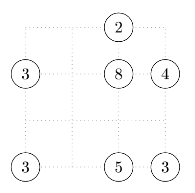
\includegraphics[width=4cm]{images/GrilleHashi}
  \caption{Grille Hashi avant résolution}
\end{figure}

Afin de résoudre une instance et de trouver une solution au problème qui se pose dans le Hashi, il faut que toutes les îles soient reliées par un nombre de ponts égal au degré de l'île concernée (degré qui sera compris entre 1 et 8, car il est impossible de placer plus), mais aussi que toute île soit accessible à partir de n'importe quelle autre île, autrement dit que le réseau soit connexe. Il ne peut cependant n'y avoir qu'un maximum de deux ponts directs entre deux îles, et ces ponts là ont pour obligation d'être soit verticaux, soit horizontaux. De même, les ponts ne peuvent pas se croiser, ou encore traverser une île et celles-ci ne peuvent être collées côte à côte. Nous noterons aussi qu'il n'existe qu'une seule et unique solution à chaque instance. (Figure 2.2) 
\newline \newline 

\begin{figure}[htp]
  \centering
  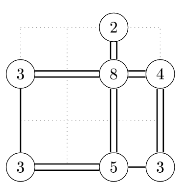
\includegraphics[width=4cm]{images/GrilleHashiResolu}
  \caption{Grille Hashi après l'application de l'unique résolution}
\end{figure}

Pour réaliser cela, nous avons dû:
\begin{itemize}
    \item définir des types de données pour représenter les données de notre problème
    \item réfléchir aux structures de données pour la résolution du casse-tête
    \item écrire des algorithmes de résolution et les programmer
    \item expérimenter les différentes méthodes
    \item faire une trace graphique de la résolution
\end{itemize}

\smallbreak
Trouver une solution à ce problème est NP-complet. NP-complet signifie que c'est un problème non-déterministe, c'est-à-dire, que nous ne pourrons pas résoudre ce casse-tête de façon polynomiale sur toutes les possibilités qu'il existe. De plus, il se peut que nous ne trouvions pas la solution du premier coup, et donc que nous soyons obligés de retenter la résolution en prenant le problème différemment. 
\smallbreak
Avant d'entrer plus en détail dans notre façon de traiter le problème, nous allons définir quelques notions. Premièrement, nous appellerons un pont simple un pont reliant les mêmes îles. De la même façon, un double pont correspond à deux ponts reliants les même îles.
\newline
Ensuite, une île sera considérée comme "résolue" lorsque son degré sera égal à son nombre de ponts. La grille du casse-tête sera elle considérée comme résolue lorsque la solution au problème sera trouvée.
\newline
Enfin, une île est considérée comme voisin possible d'une autre île si les deux peuvent être directement reliées, tandis qu'une île est considérée comme voisin réel d'une autre île si les deux sont déjà reliées. Il est important de noter cependant que dans cette façon de voir les choses, une île peut être à la fois voisin possible et réel d'une autre île (e.g. une île reliée par un pont simple sera considérée comme un voisin réel, mais restera dans les voisins possibles si elle n'est toujours pas résolue).
On appellera valeur restante d'une île, le nombre de ponts placés de l'île soustrait à son degré. Autrement dit, le nombre de ponts qu'il est encore possible de placer.
\smallbreak
Afin de trouver comment relier les îles correctement, nous avons établi des "règles" pour la création de pont: Notre première règle consiste à dire qu'une île ayant une valeur restante égale au double de son nombre de voisins possible aura un pont double entre elle et chacun de ses voisins possibles. En effet cela est le seul moyen pour l'île d'être résolue et nous permet donc de saturer ces îles là, nous ouvrant alors d'autres éventuelles possibilités sur le reste de la grille. (Figure 2.3 et 2.4)\newline

\begin{figure}[htp]
  \centering
  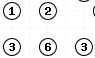
\includegraphics[width=3cm]{images/Regle1}
  \caption{Îles avant l'application de la règle 1}
\end{figure}

\begin{figure}[htp]
  \centering
  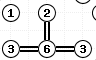
\includegraphics[width=3cm]{images/Regle1_2}
  \caption{Îles après l'application de la règle 1}
\end{figure}


Notre seconde règle consiste à dire que si la valeur restante d'une île plus un correspond au double du nombre de voisins possibles de cette même île, alors un pont simple peut être placé sur tous ses voisins possibles Dans le cas particulier où l'île et un de ses voisins possibles sont déjà reliés par un pont simple, on passe le pont simple en pont double. Cependant, cette règle ne fonctionne que sur les îles ayant un degré impair. (Figure 2.5 et 2.6)
\newline
Si à la suite de cette deuxième règle la valeur restante de l'île correspond à son nombre exact de voisins possibles, alors on "remplit" l'île, c'est à dire que nous plaçons un deuxième pont entre l'île concernée et tous ses voisins possibles, créant ainsi des ponts doubles. En effet, il se peut que le nombre de voisins possibles de l'île ait pu changer suite à la règle, et ce dans le bon sens, c'est-à-dire, de façon à ce que les deux valeurs précédents soient égales permettant alors le remplissage de l'île par des doubles ponts puisque nous rappelons que cette "règle" ne se produit qu'après l'application de la deuxième et donc qu'il y a déjà des ponts simples placés. (Figure 2.7) \newline

\begin{figure}[htp]
  \centering
  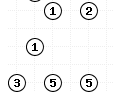
\includegraphics[width=3.5cm]{images/Regle2_1}
  \caption{Îles avant l'application de la règle 2}
\end{figure}

\begin{figure}[htp]
  \centering
  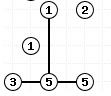
\includegraphics[width=3.5cm]{images/Regle2_2}
  \caption{Îles après l'application de la règle 2}
\end{figure}

\begin{figure}[htp]
  \centering
  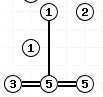
\includegraphics[width=3.5cm]{images/Regle2_3}
  \caption{Suite de la règle 2 - Cas particulier}
\end{figure}